\documentclass[12pt, letterpaper, preprint]{aastex}
\usepackage{hyperref}
\usepackage{color}
%%% This file is generated by the Makefile.
\newcommand{\giturl}{\url{https://github.com/changhoonhahn/centralMS}}
\newcommand{\githash}{9119283}\newcommand{\gitdate}{2019-04-05}\newcommand{\gitauthor}{changhoonhahn}


% typesetting shih
\linespread{1.08} % close to 10/13 spacing
\setlength{\parindent}{1.08\baselineskip} % Bringhurst
\setlength{\parskip}{0ex}
\let\oldbibliography\thebibliography % killin' me.
\renewcommand{\thebibliography}[1]{%
  \oldbibliography{#1}%
  \setlength{\itemsep}{0pt}%
  \setlength{\parsep}{0pt}%
  \setlength{\parskip}{0pt}%
  \setlength{\bibsep}{0ex}
  \raggedright
}
\setlength{\footnotesep}{0ex} % seriously?

\newcommand\tab[1][1cm]{\hspace*{#1}}
\newcommand{\todo}[1]{{\bf \textcolor{red}{#1}}}
\newcommand{\beq}{\begin{equation}}
\newcommand{\eeq}{\end{equation}}
\newcommand{\overbar}[1]{\mkern 1.5mu\overline{\mkern-1.5mu#1\mkern-1.5mu}\mkern 1.5mu}
\newcommand{\avgSFR}{\overline{\raisebox{0pt}[1.2\height]{SFR}}}
\newcommand{\SFR}{\mathrm{SFR}}
\newcommand{\fq}{f_\mathrm{Q}}
\newcommand{\fqcen}{f_\mathrm{Q}^\mathrm{cen}}
\newcommand{\zinit}{z_\mathrm{initial}}
\newcommand{\taucen}{\tau_\mathrm{Q}^\mathrm{cen}}
\newcommand{\bitem}{\begin{itemize}}
\newcommand{\eitem}{\end{itemize}}

\begin{document}\sloppy\sloppypar\frenchspacing

%\title{Central Galaxies on the Main Sequence} 
\title{Star Formation Main Sequence in a Hierarchical Universe} 
\date{\texttt{DRAFT~---~\githash~---~\gitdate~---~NOT READY FOR DISTRIBUTION}}
\author{ChangHoon~Hahn\altaffilmark{1}, 
Jeremy L.~Tinker\altaffilmark{2}, 
Andrew R.~Wetzel\altaffilmark{3,4,5}}
\altaffiltext{1}{Lawrence Berkeley National Laboratory, 1 Cyclotron Road, Berkeley, CA 94720}
\altaffiltext{2}{Center for Cosmology and Particle Physics, Department of Physics, New York University, 4 Washington Place, New York, NY 10003}
\altaffiltext{3}{TAPIR, California Institute of Technology, Pasadena, CA USA}
\altaffiltext{4}{Carnegie Observatories, Pasadena, CA USA}
\altaffiltext{5}{Department of Physics, University of California, Davis, CA USA}
\email{changhoon.hahn@lbl.gov}

\begin{abstract}
    \todo{motivation, methodology, impact.}
    In observations star forming galaxies form a tight $log\;M_*$ to $log\;SFR$ 
    relation referred to as the {\em star formation main sequence} (SFMS) out to $z\sim2$. 
    Beyond the evolution ``along'' this SFMS, however, the star formation histories of star 
    forming galaxies have not been precisely characterized. 
    The SFH of these galaxies govern SMF, SFMS, and also observed constraints on the stellar mass to halo mass
    relation. 

    By combining high-resolution cosmological $N$-body simulation with observed evolutionary 
    trends of SF galaxies, we construct a model that tracks the evolution of star forming 
    central galaxies over the redshift $z < 1$. Comparing this model 

    Observations find a remarkably small scatter in the stellar mass to halo mass relation. 
    Somehow the star formation histories of galaxies must 
    
    According to observations, star forming galaxies form a tight $log\;M_*$ to $log\;SFR$ 
    relation referred to as the ``star formation main sequence'' out to $z\sim2$. 
\end{abstract}
\keywords{methods: numerical -- galaxies: clusters: general -- 
galaxies: groups: general -- galaxies: evolution -- galaxies: haloes -- 
galaxies: star formation -- cosmology: observations.}


{\bf Checklist} 
\bitem
\item Check the correlation between halo growth rate with different $t_{delay}$ and $\delta t_{abias}$ with the total halo growth rate between $z \sim 0$ and $z \sim 1$. 
\eitem 

\section{Introduction}
\bitem 
\item Motivate why we think SF galaxies evolve along the main sequence  
\item Discuss the current thought process on galaxy assembly bias 
\item Explain the limitation of SFH derivable from observations (Claire's fisher matrix paper would be really good; ask her about the details) 
\item Observations also can't provide detail host dark matter halo properties
\item So the approach with combining observations with N-body (empirical modeling) is very effective in the context of the halo.
\item Maybe talk about how the bigger context of why this is important?  
\item Why only centrals -- because our current best understanding of satellites is that they quench after infall, so it doesn't make sense to look at them
\eitem 

\section{Central Galaxies of SDSS DR7} \label{sec:sdss}
We construct our galaxy sample following the sample selection of \cite{tinker2011}. 
We select a volume-limited sample of galaxies with $M_r −5 log(h) < −18$ and complete in
$M_* > 10^{9.4} M_\odot$ from the NYU Value-Added Galaxy Catalog \citep[VAGC;][]{blanton2005}
of the Sloan Digital Sky Survey Data Release 7~\citep[SDSS DR7;][]{abazajian2009} at 
$z \approx 0.04$. The stellar masses of these galaxies are estimated using the
$\mathtt{kcorrect}$ code~\citep{blanton2007} assuming a~\cite{chabrier2003} initial
mass function. The star formation of the galaxies are estimated spectroscopically using the
specific star formation rates (SSFR) from the current release of the MPA-JHU spectral 
reductions\footnote{http://wwwmpa.mpa-garching.mpg.de/SDSS/DR7/}~\citep{brinchmann2004}.
Generally speaking, $\mathrm{SSFR} > 10^{-11}\mathrm{yr}^{-1}$ are derived from 
$\mathrm{H}_\alpha$ emission, $10^{-11} > \mathrm{SSFR} > 10^{-12}\mathrm{yr}^{-1}$
are derived from a combination of emission lines, and $\mathrm{SSFR} < 10^{-12}\mathrm{yr}^{-1}$
are based on $D_n 4000$~\citep[see discussion in][]{wetzel2013}. We note that 
$\mathrm{SSFR} < 10^{-12}\mathrm{yr}^{-1}$ should only be considered upper limits 
to the true galaxy SSFR~\citep{salim2007}.

From our galaxy sample, we identify the central galaxies using the \cite{tinker2011} halo-based 
group-finding algorithm, which is based on the~\cite{yang2005} algorithm and tested 
in~\cite{campbell2015}. The algorithm assigns a probability of being a satellite 
galaxy, $P_\mathrm{sat}$, to each galaxy in the sample. Galaxies with $P_\mathrm{sat} \geq 0.5$ 
are classified as satellites and $P_\mathrm{sat} < 0.5$ are classified as centrals. 
In this paper we focus on central galaxies. In any group finding algorithm, galaxies are 
misassigned due to projection effects and redshift space distortions. The purity 
of the full central galaxy sample is $\sim 90\%$ with a completeness of $\sim 95\%$~\citep{tinker2017}.
Furthermore, \cite{campbell2015} find that the algorithm robustly identifies red and blue centrals
as a function of stellar mass, which is highly relevant to our analysis.  

In the left panel of Figure~\ref{fig:groupcat}, we plot the SFR-$M_*$ distribution of
the SDSS DR7 central galaxies. In the right panel, we plot the distribution of SSFR, 
$p(\log \mathrm{SSFR})$, for galaxies with $10.6 < \log \,M_* < 10.8$ (stellar mass range 
highlighted on the left panel). Both panels of Figure~\ref{fig:groupcat} illustrate the 
bimodality in the galaxy sample. The SFR-$M_*$ distribution also illustrate the correlation
between SFR and $M_*$ in star-forming galaxies \emph{i.e.} the star-formation main sequence 
(SFMS).

\subsection{Simulated Central Galaxies}
We're interesting in constructing a model that tracks central galaxies and their star 
formation within the heirarchical growth of their host halos. This requires a cosmological 
$N$-body simulation that accounts for the complex dynamical processes that govern the host 
halos of galaxies. In this paper we use the high resolution $N$-body simulation 
from~\cite{wetzel2013} generated using the \cite{white2002} $\mathtt{TreePM}$ code 
with flat $\Lambda$CDM cosmology 
($\Omega_m =0.274, \Omega_b = 0.0457, h = 0.7, n=0.95, \mathrm{and} \sigma_8 = 0.8$).
$2048^3$ particles with mass of $1.98 \times 10^8\,M_\odot$ are evolved in a $250 \mathrm{Mpc}/h$
with a Plummer equivalent smoothing of $2.5\,\mathrm{kpc}/h$ from initial conditions at $z = 150$ 
generated using second-order Lagrangian Perturbation Theory. For a more detailed description of 
the simulation, we refer readers to \cite{wetzel2013, wetzel2014}.

From the $\mathrm{TreePM}$ $N$-body simulation, `host halos' are identified using the
Friends-of-Friends (FoF) algorithm of \cite{davis1985} with linking length of $b = 0.168$
times the mean inter-partcile spacing. Within these host halos, \cite{wetzel2013} identifies  
`subhalos' as overdensities in phase space through a six-dimensional FoF 
algorithm~\citep[FoF6D][]{white2010}. The host halos and subhalos are then tracked across 
the $45$ simulation outputs from $z = 10$ to $0$ to build merger trees~\citep{wetzel2009,wetzel2010}. 
The most massive subhalos in newly-formed host halos at a given simulation output are defined 
as the `central' subhalo. A central subhalo retains its `central' definition until it falls into 
a more massive host halo. At this point it becomes a `satellite' subhalo. 

Each subhalo is assigned a $M_\mathrm{peak}$, the maxmum host halo mass that a it ever had 
as a central subhalo. Using $M_\mathrm{peak}$, a galaxy catalog is constructed from 
the subhalos using subhalo abundance matching~\citep[SHAM;][]{vale2006,yang2009,wetzel2012,wetzel2013,wetzel2014,hahn2017a}\todo{citations conroy2006, leja2013}. 
In principle, SHAM assumes a one-to-one mapping that preserves the rank ordering between subhalo $M_\mathrm{peak}$
and galaxy stellar mass $M_*$: $n(> M_\mathrm{peak}) > n(> M_*)$. Using this mapping, we can 
assign galaxy stellar mass to subhalos based on observed stellar mass functions (SMFs) at the
redshifts of the simulation outputs (snapshots). By assigning galaxy $M_*$ independently at each 
snapshot, we not only track the evolution of subhalos, but also the evolution of the galaxies' $M_*$. 

In our SHAM prescription, we use the SMF from \cite{li2009} at $z = 0.05$ and interpolate at
higher redshifts between the \cite{li2009} SMF and the SMF from \cite{marchesini2009} at 
$z = 1.6$. We choose the \cite{li2009} SMF because it is based on the same SDSS NYU-VAGC 
sample as our SDSS DR7 group catalog (see Section~\ref{sec:sdss}). We choose the 
\cite{marchesini2009} SMF, amongst others, because it produces interpolated SMFs that
monotonically increase at $z < 1$. As noted in \cite{hahn2017}, 
at $z \approx 1$, the SMF interpolated between the \cite{li2009} and \cite{marchesini2009} 
SMFs is consistent with more recent measurements from \cite{muzzin2013} and \cite{ilbert2013}. 
In this paper, as we describe later in this section, we are only interested in the snapshots 
at $z \approx 1$ and $0.05$. 

While SHAM in principle assumes a one-to-one mapping, observations find a significant
scatter in this stellar mass to halo mass mapping ($\sigma_{\log M_*}$). \cite{gu2016} 
compile 
Hence, when we use SHAM to construct our galaxy catalogs, we apply a $0.2$ dex log-normal 
scatter in $M_∗$ at fixed $M_\mathrm{peak}$. 

In Section~\ref{app:z1}, 

%In Figure 1, we illustrate the evolution of the SMFs that we use for our SHAM prescription (solid) for z = 0.05, 0.5, and 0.9. Recently, using PRIMUS, Moustakas et al. (2013) found little evolution in the SMF for z < 1 at all mass ranges. Although previous works such as Bundy et al. (2006) find otherwise. To ensure that our results do not depend on our choice of the SMFs, later in §5.2, we repeat our analysis using SMFs with no evolution (i.e. Li & White 2009 SMF throughout 0 < z < 1) and with “extreme” evolution for z > 0.05 (dash-dotted in Fig- ure 1), in which the amplitude of the SMF at z = 1.2 is approximately half the amplitude of the fiducial SMF at z = 1.2. Furthermore, while the simplest version of SHAM assumes a one-to-one correspondence between Mpeak and M∗, observations suggest that there is a scat- ter of ∼ 0.2 dex in this relation (Zheng et al. 2007; Yang et al. 2008; More et al. 2009; Gu et al. 2016). Hence, we apply a 0.2 dex log-normal scatter in M∗ at fixed Mpeak in our SHAM prescription at each snapshot inde-
%pendently.
%So far, we have subhalos populated with galaxies and their stellar mass at each of the 15 simulation outputs spanning the redshift 0.05 < z < 1. For our sample, we restrict ourselves to galaxies classified as centrals by the simulation. And also to ones that are in both the z ∼ 0.05 and z ∼ 1 snapshots. This removes < 3% of central galaxies with M∗ > 109.5 M⊙ in the z ∼ 0.05 snapshot. Our sample inevitably includes “back splash” or “ejected” satellite galaxies (Wetzel et al. 2014), mis- classified as centrals. Excluding these galaxies, however, has a negligible impact on our results. We also note that while we do not have an explicit prescription for stellar mass growth from mergers, based on SHAM, the stellar mass growth traces the merger induced subhalo growth. As we discuss later in detail, mounting evidence disfavor merger driven quenching as the trigger of star formation quenching, so our treatment of mergers do not impact our quenching timescale results. In summary, we con- struct from our simulation a catalog of central galaxies whose stellar mass and halo mass is be traced through the redshift range 0.05 < z < 1.

\subsection{Selecting $z \sim 0$ Star Forming Central Galaxies}  
\bitem
\item Describe how $f_{SFMS}$ is calculated. Reference to Tjitske in prep 
\item Then explain how it's not circular because the integrated $M_*$ has to reproduce the same SMF
\eitem

\subsection{Evolving along the Main Sequence} 
\bitem
\item Talk about the SFR and $M_*$ prescriptions 
\item parameterization of SFMS 
\item explicitly talk about the free parameters of the model. 
\item priors for $\beta_M$ and $\beta_z$ encompass the observable constraints 
\item talk about inference using ABC
\eitem

\section{Results}
\subsection{The duty cycle of star formation}
\bitem
\item Figure that illustrates the fit to observables 
\item Figure of sigma M star as a function of duty cycle compared to observations 
\eitem 

\subsection{The need for a galaxy assembly bias}
\bitem
\item discuss how $t_{duty}$ is not enough to be consistent with $\sigma_{M_*}$. 
\item first clarify what you mean by galaxy assembly bias 
\item discuss implementation of galaxy assembly bias
\item Figure (pedagogical) of dlogSFR versus dMh dt for different correlation amounts 
\item Figure of different tdelay and dtabias 
\item Figure of sigma M star as a function of duty cycle and realistic dt abias and t delay 
\eitem

\section{Discussion} \label{sec:discussion}
\subsection{Rethinking the Main Sequence?}
\bitem 
\item Test the SMHMR for Louis's SFHs 
\eitem 

\section{Summary} \label{sec:summary}


\appendix
\section{$z \sim 1$ observations} \label{app:z1}
Much of the results presented in this paper are based on comparison 
between our model and observations at $z \sim 0.$. Our model is initalized 
at $z \sim 1$. Therefore, in this section we test some of the choices 
we make in our intializations. 

\bitem
\item Test impact of $z \sim 1$ SMF
\item Test impact of $z \sim 1$ $\sigma_{\log M_*}$ 
\eitem

\begin{figure}
\begin{center}
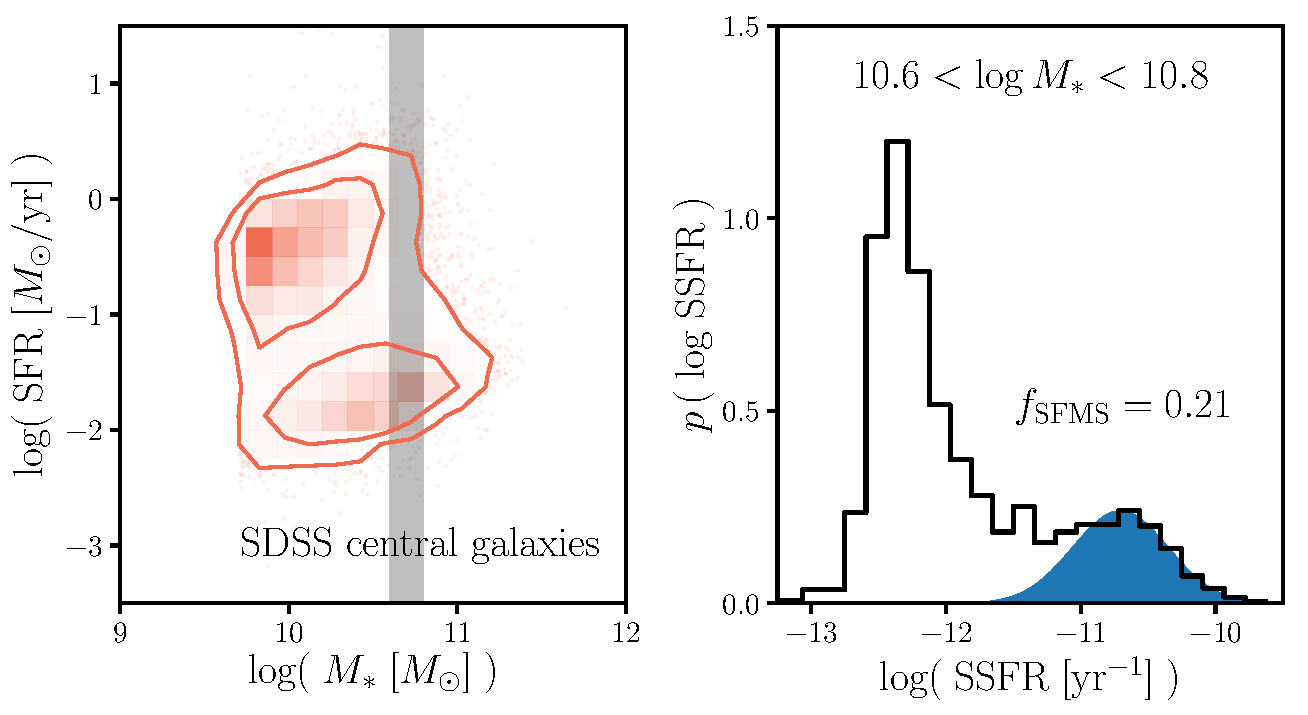
\includegraphics[width=0.9\textwidth]{figs/groupcat.pdf}
\caption{SDSS DR7 Group Catalog. Fitting of the SFMS.}
\label{fig:groupcat}
\end{center}
\end{figure}

\begin{figure}
\begin{center}
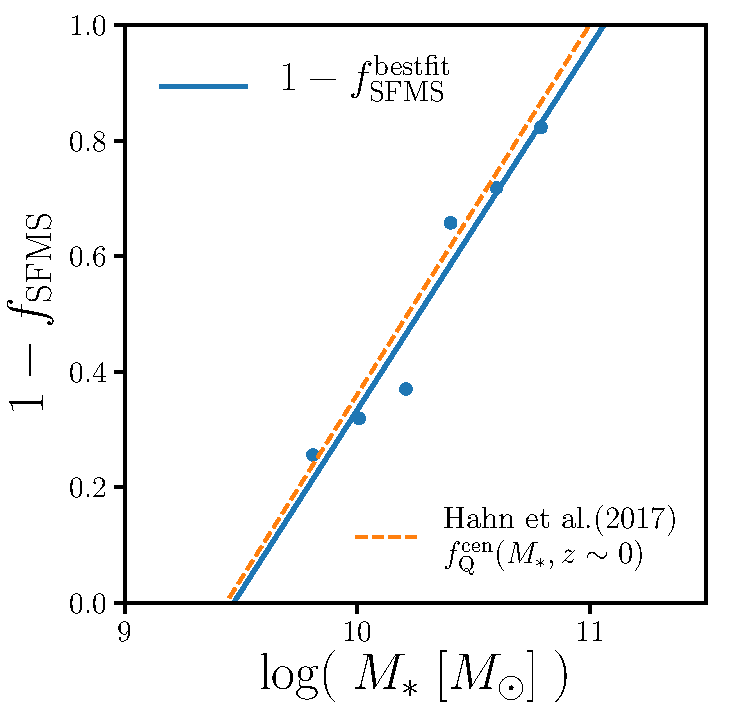
\includegraphics[width=0.5\textwidth]{figs/fq_fsfms.pdf}
\caption{SFMS fraction versus quiescent fraction from Hahn}
\label{fig:fq_fsfms}
\end{center}
\end{figure}

\begin{figure}
\begin{center}
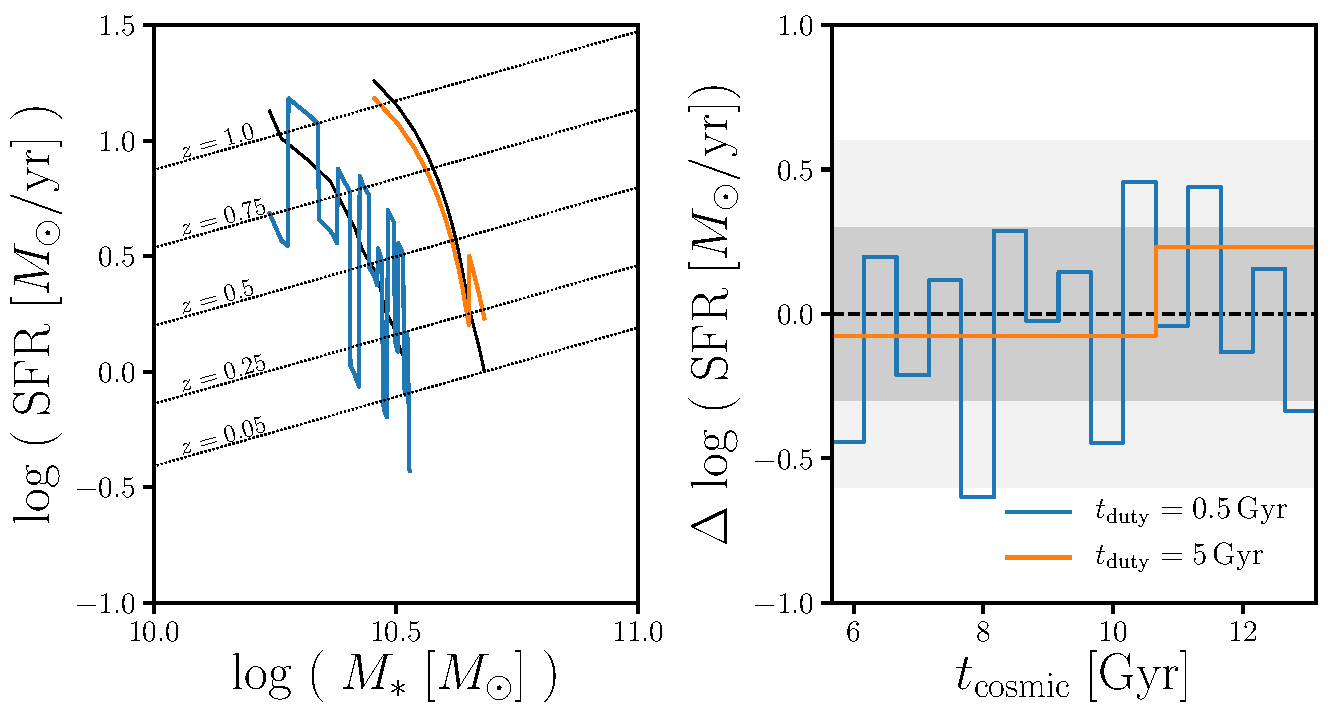
\includegraphics[width=0.9\textwidth]{figs/sfh_pedagogical.pdf}
\caption{Pedagogical figure that illustrates how star forming central galaxies in our model
evolve along the SFMS.}
\label{fig:sfh_model}
\end{center}
\end{figure}

\begin{figure}
\begin{center}
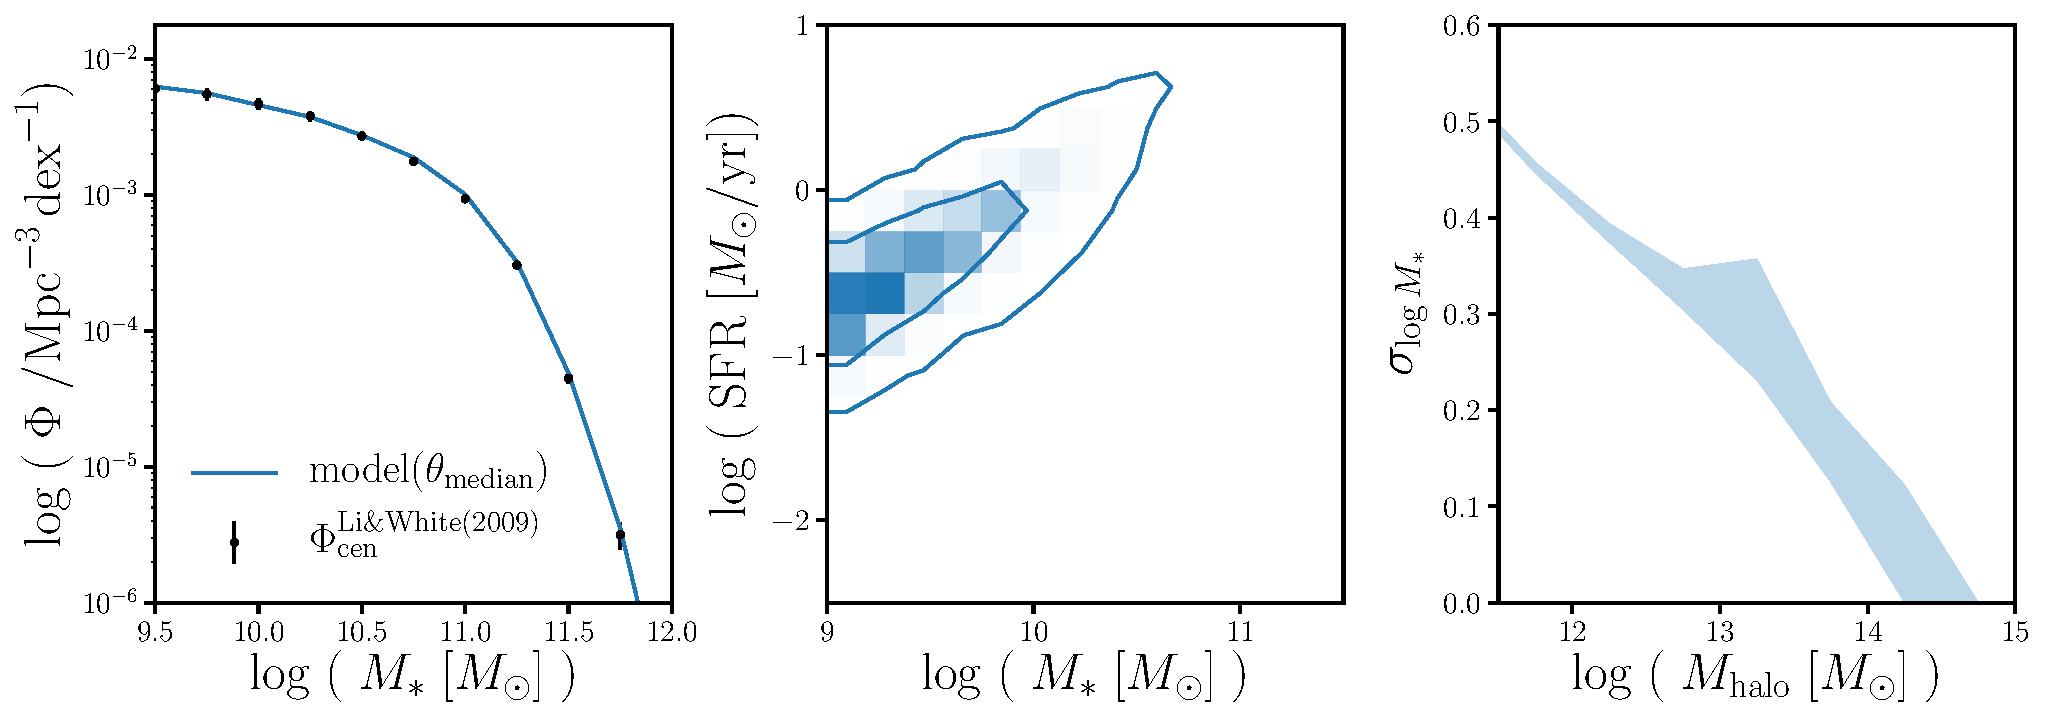
\includegraphics[width=0.9\textwidth]{figs/qaplot_abc_test0_t14.pdf}
%qaplot_abc_test0_t14.pdfqaplot_abc_randomSFH_short_t9.pdf}
\caption{}
\label{fig:abc_demo}
\end{center}
\end{figure}

\begin{figure}
\begin{center}
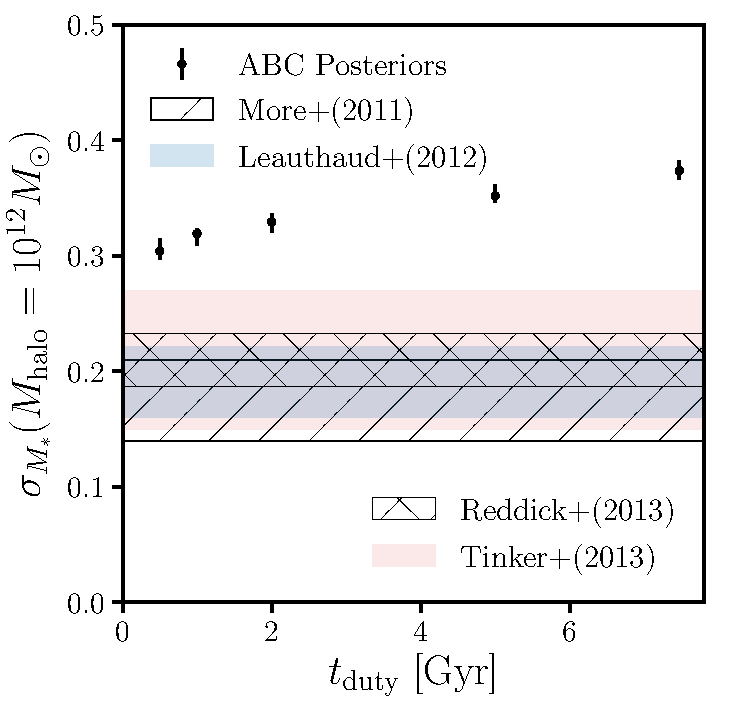
\includegraphics[width=0.5\textwidth]{figs/sigMstar_tduty.pdf}
\caption{}
\label{fig:abc_demo}
\end{center}
\end{figure}

%%%%%%%%%%%%%%%%%%%%%%%%%%%%%%%%%%%%%%%%%%%%%%%%%%%%%%%%%%%%%%%
% Acknowledgements
%%%%%%%%%%%%%%%%%%%%%%%%%%%%%%%%%%%%%%%%%%%%%%%%%%%%%%%%%%%%%%%
\section*{Acknowledgements}
Louis Abramson

\bibliographystyle{yahapj}
\bibliography{centralMS}
\end{document}
